\begin{frame}{Computability of Total Functions on $\Reals$}
    \begin{center}
        
\includegraphics[width=.88\linewidth]{total.png}
    \end{center}
\end{frame}
% \begin{frame}{Computability of Partial Functions on $\Reals$}
%     \begin{center}
%         
\includegraphics[width=.88\linewidth]{partial.png}
%     \end{center}
% \end{frame}
\begin{frame}{Computability of Total Functions on $\Reals$}
        \begin{center}
        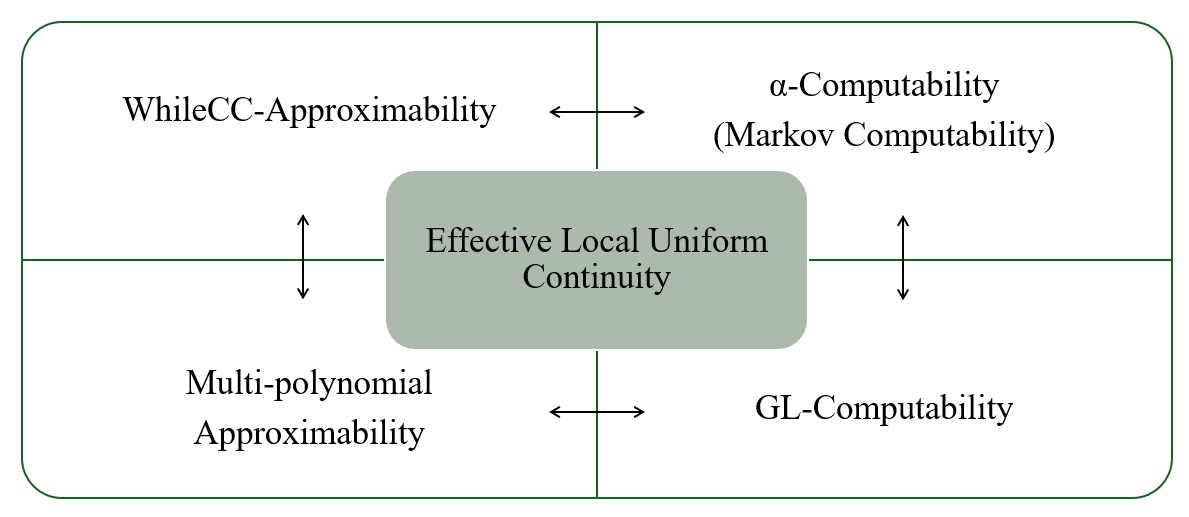
\includegraphics[width=.6\linewidth]{total-zoomed.png}
    \end{center}
\end{frame}

\begin{frame}{Computability of Partial Functions on $\Reals$}
    \textbf{For partial functions on $\Reals$}, \citet{ModelOfCompForPartFunc_MingQuanFuAndJeffZucker} generalize effectively locally uniform continuity to \textbf{\textcolor{violet}{acceptability}} to get an equivalence.\\
    \pause
     \begin{exampleblock}{\textbf{\textcolor{BrickRed}{Problem}}}
        How general is this class of acceptable functions?
     \end{exampleblock}
     \pause
    \begin{center}
        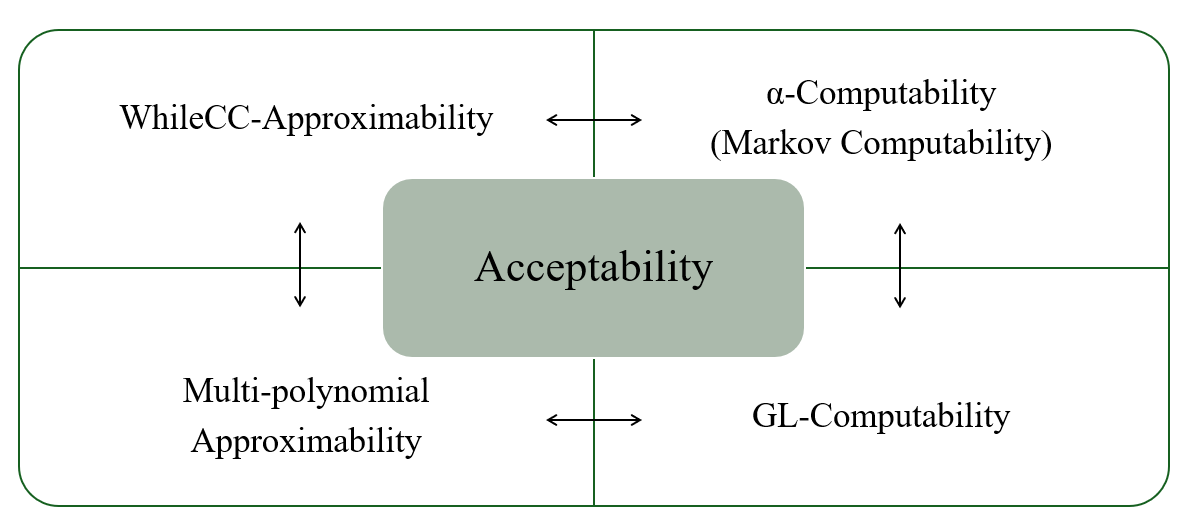
\includegraphics[width=.6\linewidth]{partial-zoomed.png}
    \end{center}
     \begin{exampleblock}{\color{OliveGreen}\textbf{Useful First Step Towards Solution}}
         Show that the elementary functions satisfy the acceptability conditions. 
     \end{exampleblock}
\end{frame}


 